


\documentclass[11pt,twoside]{article}\usepackage[]{graphicx}\usepackage[table]{xcolor}
% maxwidth is the original width if it is less than linewidth
% otherwise use linewidth (to make sure the graphics do not exceed the margin)
\makeatletter
\def\maxwidth{ %
  \ifdim\Gin@nat@width>\linewidth
    \linewidth
  \else
    \Gin@nat@width
  \fi
}
\makeatother

\definecolor{fgcolor}{rgb}{0.345, 0.345, 0.345}
\newcommand{\hlnum}[1]{\textcolor[rgb]{0.686,0.059,0.569}{#1}}%
\newcommand{\hlsng}[1]{\textcolor[rgb]{0.192,0.494,0.8}{#1}}%
\newcommand{\hlcom}[1]{\textcolor[rgb]{0.678,0.584,0.686}{\textit{#1}}}%
\newcommand{\hlopt}[1]{\textcolor[rgb]{0,0,0}{#1}}%
\newcommand{\hldef}[1]{\textcolor[rgb]{0.345,0.345,0.345}{#1}}%
\newcommand{\hlkwa}[1]{\textcolor[rgb]{0.161,0.373,0.58}{\textbf{#1}}}%
\newcommand{\hlkwb}[1]{\textcolor[rgb]{0.69,0.353,0.396}{#1}}%
\newcommand{\hlkwc}[1]{\textcolor[rgb]{0.333,0.667,0.333}{#1}}%
\newcommand{\hlkwd}[1]{\textcolor[rgb]{0.737,0.353,0.396}{\textbf{#1}}}%
\let\hlipl\hlkwb

\usepackage{framed}
\makeatletter
\newenvironment{kframe}{%
 \def\at@end@of@kframe{}%
 \ifinner\ifhmode%
  \def\at@end@of@kframe{\end{minipage}}%
  \begin{minipage}{\columnwidth}%
 \fi\fi%
 \def\FrameCommand##1{\hskip\@totalleftmargin \hskip-\fboxsep
 \colorbox{shadecolor}{##1}\hskip-\fboxsep
     % There is no \\@totalrightmargin, so:
     \hskip-\linewidth \hskip-\@totalleftmargin \hskip\columnwidth}%
 \MakeFramed {\advance\hsize-\width
   \@totalleftmargin\z@ \linewidth\hsize
   \@setminipage}}%
 {\par\unskip\endMakeFramed%
 \at@end@of@kframe}
\makeatother

\definecolor{shadecolor}{rgb}{.97, .97, .97}
\definecolor{messagecolor}{rgb}{0, 0, 0}
\definecolor{warningcolor}{rgb}{1, 0, 1}
\definecolor{errorcolor}{rgb}{1, 0, 0}
\newenvironment{knitrout}{}{} % an empty environment to be redefined in TeX

\usepackage{alltt}
\usepackage[a4paper, inner=2cm, outer=2cm, top=2cm, bottom=3cm]{geometry}

\usepackage[utf8]{inputenc} 
\usepackage[T1]{fontenc}
\usepackage[sort&compress]{natbib}
\usepackage[french]{babel}

\addto\captionsfrench{\def\tablename{Tableau}}
\addto\captionsfrench{\renewcommand*{\contentsname}{Sommaire:}}
\addto\captionsfrench{%
  \renewcommand{\listfigurename}{Liste des figures:}%
  \renewcommand{\listtablename}{Liste des tableaux:}%
  \renewcommand{\abstractname}{Résumé}%
}
\usepackage{caption}
\usepackage[labelsep=endash]{caption}
\usepackage{graphicx}
\usepackage{colortbl}
\usepackage{booktabs}
\usepackage{longtable}
\usepackage{array}
\usepackage{multirow}
\usepackage{wrapfig}
\usepackage{float}
\usepackage{pdflscape}
\usepackage{tabu}
\usepackage{threeparttable}
\usepackage{threeparttablex}
\usepackage[normalem]{ulem}
\usepackage{makecell}
\usepackage[table]{xcolor}
\usepackage{ae,aeguill}
\usepackage{subcaption}
\usepackage{csquotes}


% Colonne centrée horizontalement avec largeur fixe
\newcolumntype{C}[1]{>{\centering\arraybackslash}p{#1}}

% Optionnel : colonne alignée à droite
\newcolumntype{R}[1]{>{\raggedleft\arraybackslash}p{#1}}

% Colonne alignée à gauche (par défaut)
\newcolumntype{L}[1]{>{\raggedright\arraybackslash}p{#1}}

\usepackage{authblk}
\renewcommand\Authand{ et }
\renewcommand\Authands{ et }

\usepackage{textcomp}
\usepackage{hyperref}
\pdfstringdefDisableCommands{%
  \def\\{}%
  }
\hypersetup{ 
colorlinks=true, 
linkcolor=blue, 
citecolor=blue, 
filecolor=blue, 
urlcolor=blue, 
pdftitle= {Suivi des poissons migrateurs de la Béthune par vidéo-comptage au moulin d'Archelles,\\ année 2025 }, pdfauthor={Jean-Philippe Hanchard},
pdfsubject={stacomi},
 pdfkeywords={stacomi} {migrateurs} {Béthune} {poissons}
}
\pdfoptionpdfminorversion=7
\renewcommand{\sectionmark}[1]{\markboth{}{\emph{\thesection~#1}}}
\renewcommand{\subsectionmark}[1]{\markboth{}{\emph{\thesubsection~#1}}}
\renewcommand{\subsubsectionmark}[1]{\markboth{}{\emph{\thesubsection~#1}}}

\makeatletter
    \def\@@and{et}
\makeatother

\makeatletter
\pretocmd\abstract{\hrule\vspace{1em}}{}{}
\makeatother

\usepackage{fancyhdr}
\pagestyle{fancy}
\fancyhf{}
\rhead{\rightmark}
\lfoot{\footnotesize{Suivi des poissons migrateurs de la Béthune par vidéo-comptage au moulin d'Archelles, année 2025}} %Insere un pied de page avec le texte a gauche.
\rfoot{\thepage}
\setlength{\headheight}{15pt}

\usepackage{pdfpages}
\usepackage{setspace}
\onehalfspacing

% Définition des couleurs
\definecolor{bleuTitre}{RGB}{0,70,140} % Bleu profond
\definecolor{grisBloc}{RGB}{240,240,240} % Gris clair

%%%%%%%%%%%%%%%%%%%%%%%%%%%%%%%%%%%%%%%%%%%
%%%%%% CHUNK DE CHARGEMENT INITIAL  %%%%%%%
%%%%%%%%%%%%%%%%%%%%%%%%%%%%%%%%%%%%%%%%%%%


























%% Makes a path to your graphics' folder.
\graphicspath{{image/}}

\title{Suivi des poissons migrateurs sur les STACOMI du bassin de la Seine,
année 2025}

\author[1]{Jean-Philippe Hanchard}
\author[1]{Sébastien Grall}

\affil[1]{Seine-Normandie Migrateurs, 40 avenue Robert Hooke 76800 Saint-Étienne-du-Rouvray}
\date{}
\IfFileExists{upquote.sty}{\usepackage{upquote}}{}
\begin{document}

\hypersetup{pageanchor=false}

\begin{titlepage}

   \centering

    % --- Bandeau supérieur avec logos ---
    \begin{minipage}{\textwidth}
        \centering
        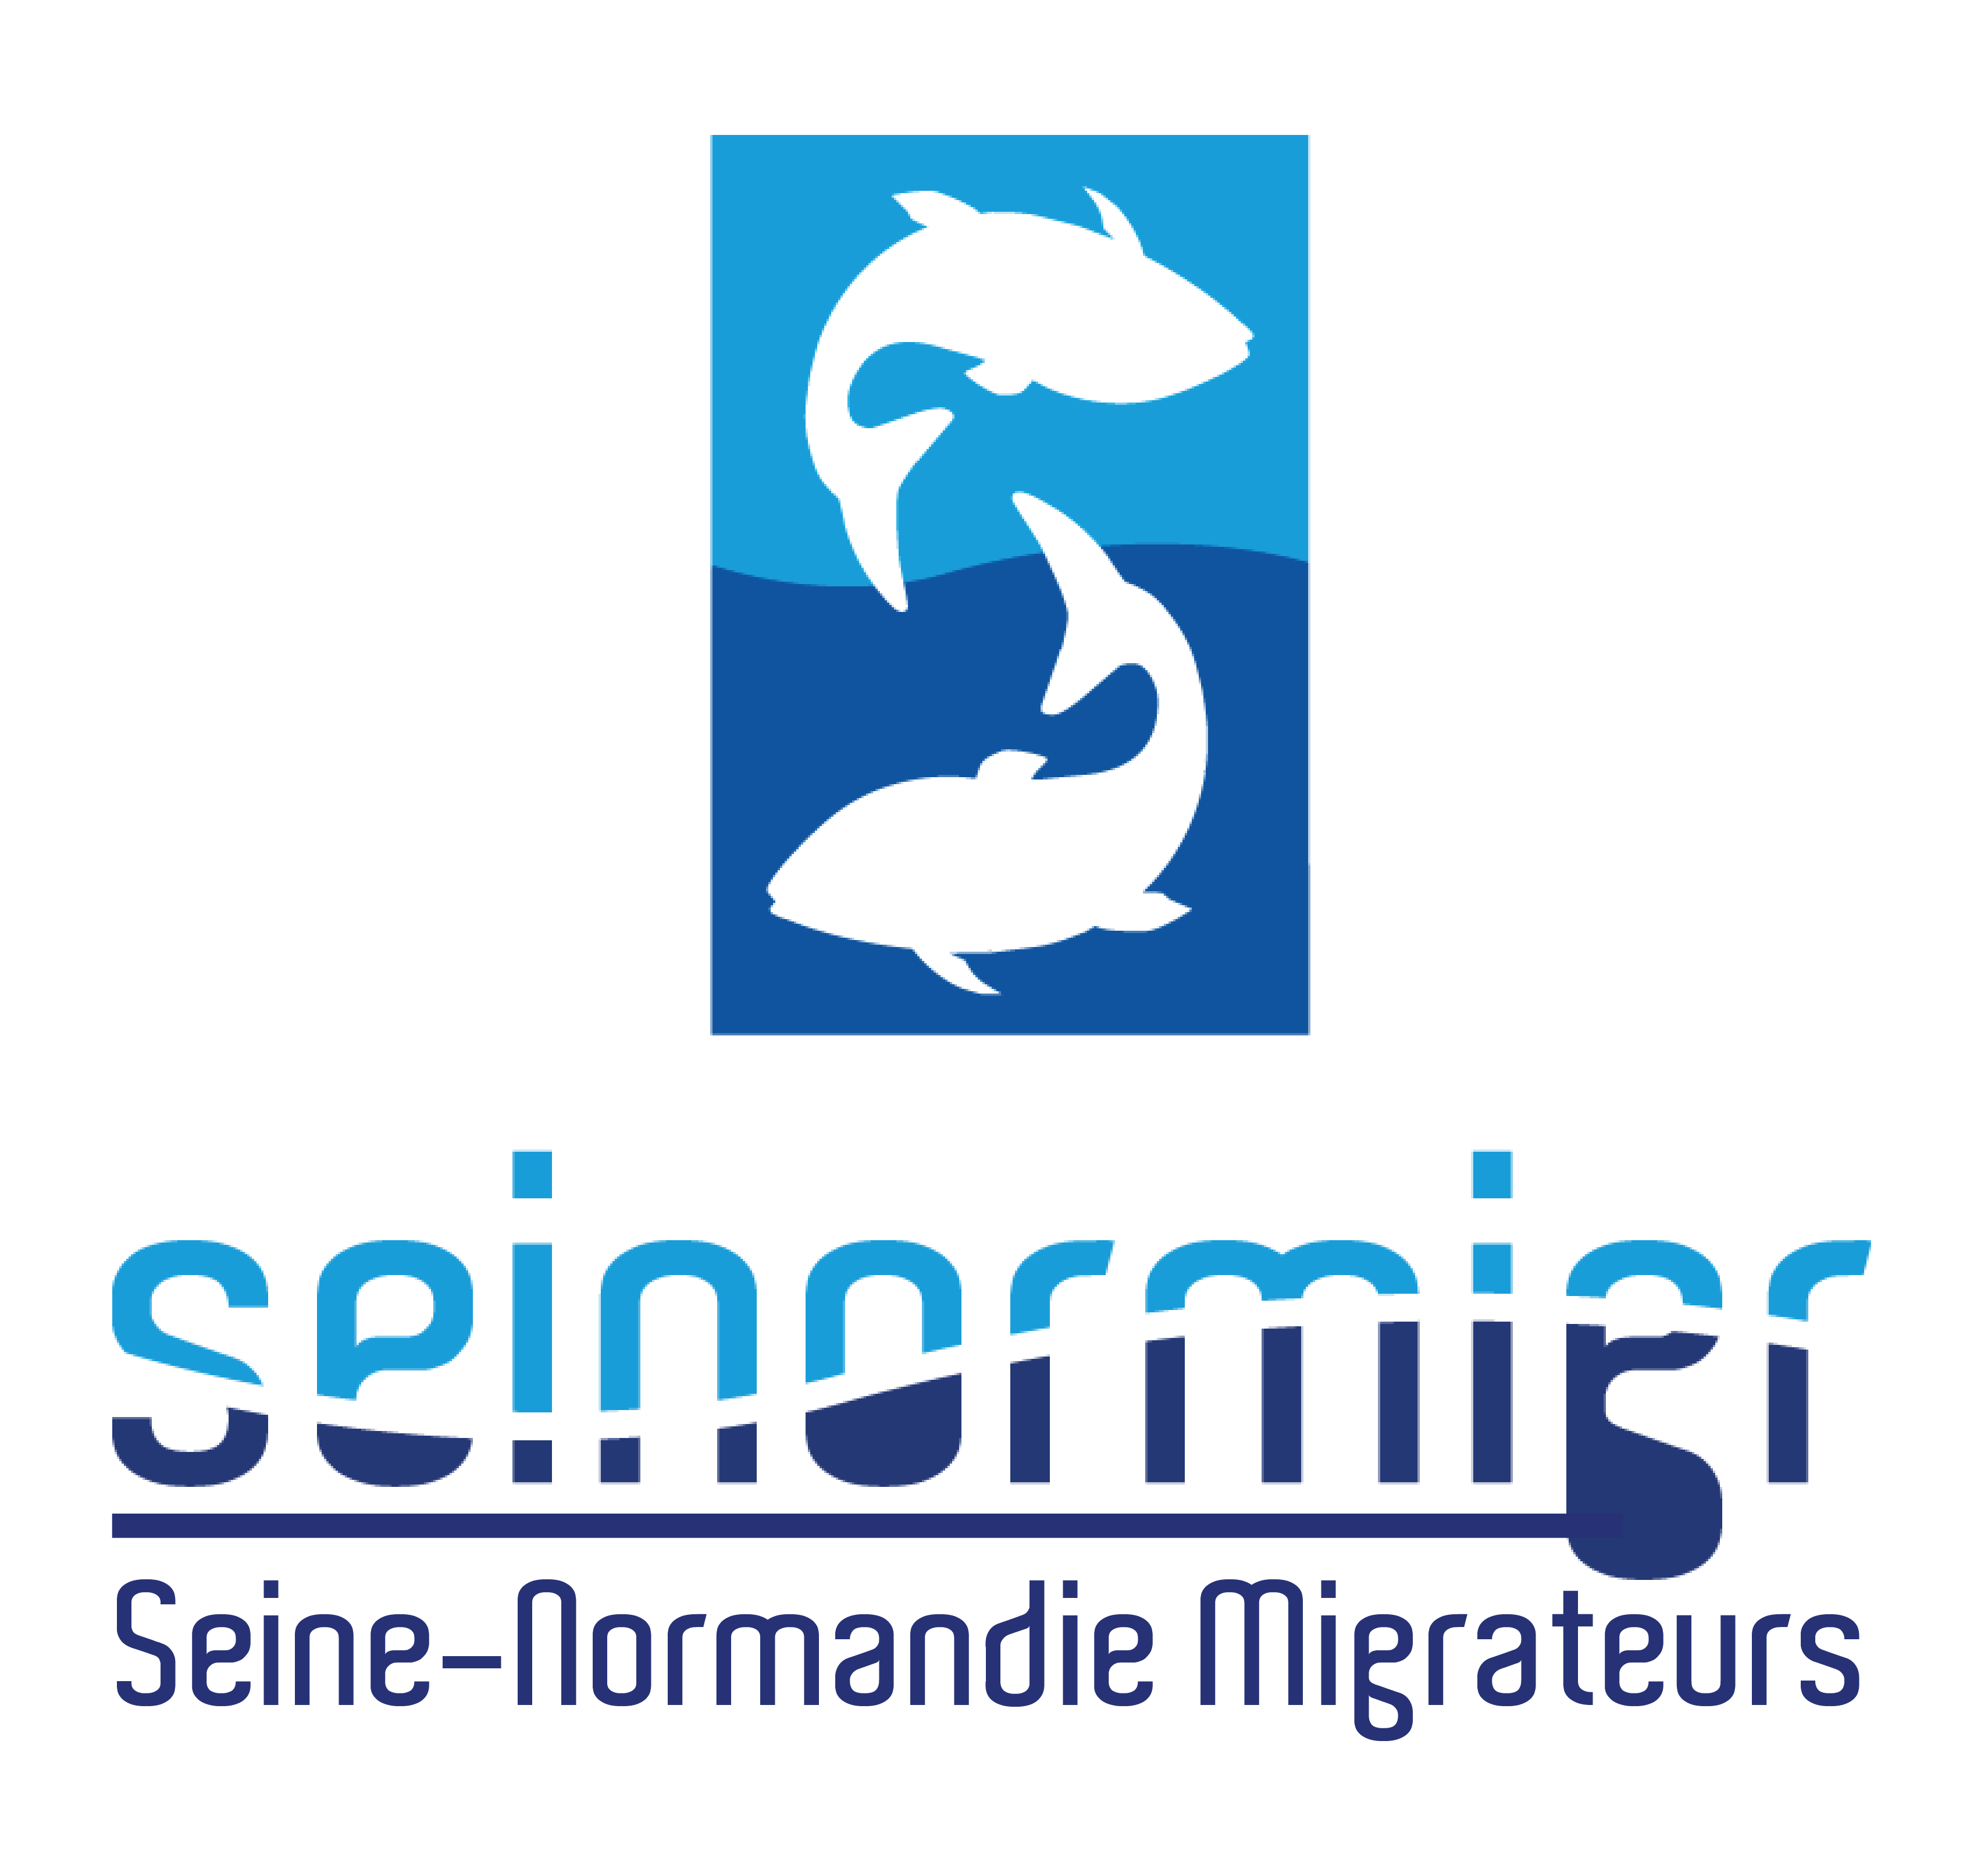
\includegraphics[height=4cm]{logos/logo_seinormigr.png}\hspace{1cm}
    \end{minipage}
    \vspace{1.5cm}
    
        \begin{minipage}{\textwidth}
        \centering
        
\includegraphics[height=1.5cm]{logos/logo_fnpf.png}\hspace{1cm}
        % \includegraphics[height=1.5cm]{logos/logo_vnf.jpg}\hspace{1cm}
        % \includegraphics[height=1.5cm]{logos/logo_hydrowatt.jpg}\hspace{1cm}
        % \includegraphics[height=1.5cm]{logos/logo_semao.png}
    \end{minipage}
    \vspace{1.5cm}

    % --- Bandeau bleu pour le titre ---
    \colorbox{bleuTitre}{
        \parbox{\textwidth}{
            \centering
            \vspace{0.5cm}
            {\Huge \textbf{\textcolor{white}{Suivi des poissons migrateurs de la Béthune par vidéo-comptage au moulin d'Archelles}}}\par
            \vspace{0.3cm}
            {\LARGE \textbf{\textcolor{white}{Année 2025}}}\par
            \vspace{0.3cm}
        }
    }
    \vspace{2cm}

    % --- Bloc Association avec fond gris ---
    \colorbox{grisBloc}{
        \parbox{0.9\textwidth}{
            \centering
            \vspace{0.5cm}
            {\Large \textbf{Seine-Normandie Migrateurs}}\par
            \vspace{0.3cm}
            \textit{Association interrégionale pour la restauration et la gestion des populations de poissons migrateurs}\par
            \vspace{0.5cm}
        }
    }
    \vspace{1.5cm}

    % --- Coordonnées ---
    \begin{spacing}{1.2}
    \textbf{Adresse :} 40 avenue Robert Hooke - 76800 Saint-Étienne-du-Rouvray\par
    %\textbf{Tél :} 02 35 62 01 55 \quad \textbf{Fax :} 02 35 62 01 72\par
    \textbf{Email :} seinormigr@gmail.com \quad \textbf{Site :} www.seinormigr.fr
    \end{spacing}

    \vfill
    % --- Bandeau inférieur avec logos partenaires ---
    \begin{minipage}{\textwidth}
        \centering
        
\includegraphics[height=2cm]{logos/LOGO RF AESN_RVB.png}\hspace{1cm}
        
\includegraphics[height=2cm]{logos/logo_fnpf.png}
    \end{minipage}

\end{titlepage}


\newpage
\thispagestyle{empty}
\strut

\newpage

\pagenumbering{roman} \setcounter{page}{1}

\maketitle

\begin{abstract}




% Les poissons migrateurs entrant dans l'estuaire de la Seine sont contrôlés au niveau du barrage de Poses, marquant la fin de l'estuaire. Cette ouvrage est équipé de dispositifs de franchissement piscicole et de comptage sur les deux rives. Les individus s'engageant sur l'axe Oise peuvent ensuite être observés au barrage de Pontoise, équipé d'un système de vidéocomptage depuis 2023. Un dernier point de contrôle est positionné sur l'Aisne, au barrage de Carandeau depuis 2018.
% Les effectifs comptabilisés en annee sur l'ensemble de ces stations sont présentés dans le tableau \ref{tab:recap}. Les valeurs négatives correspondent à des individus dévalants enregistrés lors du vidéocomptage.
% 
% \input{table/recap.tex}

\end{abstract}

\newpage
\begin{singlespace}

\tableofcontents

\clearpage

\listoffigures

\listoftables

\hypersetup{pageanchor=false}

\clearpage
\end{singlespace}

\pagenumbering{arabic} \setcounter{page}{1} 

\section{Introduction}

La situation de l'ensemble des poissons migrateurs dans le monde
est similaire : le nombre de populations,
les aires de répartition et les abondances sont en déclin depuis la fin du 19\up{e} siècle
\citep{saunders_atlantic_1981,bagliniere_reintroductions_1990,parrish_why_2011,jonsson_extinction_1999,
keith_atlas_2001,rochard_identification_2007,limburg_dramatic_2009}.
Le besoin de ces espèces de migrer entre différents habitats, essentiels à la finalisation
de leur cycle biologique, implique une vulnérabilité particulière face aux perturbations de l'environnement.
Aujourd'hui, la majorité des poissons amphihalins figurent dans la liste rouge
des espèces menacées de l'IUCN \citep{limburg_dramatic_2009}.

Sur la Seine, le constat est analogue. Historiquement, 10 espèces amphihalines dont 8 poissons grands migrateurs,
fréquentaient le fleuve sur presque l'ensemble de son bassin versant \citep{moreau_histoire_1881,moreau_les_1898,
poplin_peuplement_1952,euzenat_migren_1992,rochard_identification_2007}, souvent en abondance. Toutefois, sous l’effet d’une anthropisation croissante du fleuve, le déclin a commencé dès les années 1850. Les dégradations sont multiples et semblables à ce qui a été démontré sur d'autres systèmes fluviaux
\citep{nehlsen_pacific_2011,mcdowall_different_1999,lichatowich_depletion_1999,mckinnell_spatial_1999,
limburg_dramatic_2009}. L'édification de barrages, la chenalisation, la pollution, la dégradation des habitats et la surpêche ont conduit au cours du 20\up{ème} siècle à l'extinction locale des derniers grands migrateurs sur le bassin de la Seine
\citep{euzenat_migren_1992,belliard_peuplement_1994,mouchel_bassin_1998,boet_multiple_1999,rochard_identification_2007},
seule l'Anguille européenne subsistait encore à cette période \citep{boet_multiple_1999,rochard_identification_2007}.

Néanmoins, les efforts entrepris dans le traitement des effluents anthropiques, notamment ceux de l'agglomération parisienne, durant ces deux dernières décennies ont contribué à la franche amélioration de la qualité de l'eau de la Seine \citep{billen_programme_1999,belliard_return_2009,
gousailles_limpact_2009}.
Cette amélioration s’est rapidement traduite par le retour des poissons amphihalins, incluant plusieurs espèces estuariennes telles que \href{https://seinormigr.fr/fr/petits-migrateurs-d332}{l’Éperlan} (\textit{Osmerus eperlanus}), \href{https://seinormigr.fr/fr/petits-migrateurs-d332}{le Flet commun} (\textit{Platichthys flesus}) et \href{https://seinormigr.fr/fr/petits-migrateurs-d332}{le Mulet porc} (\textit{Chelon ramada}). Par ailleurs, un retour progressif des six espèces constituant la communauté historique des grands poissons migrateurs de la Seine est également observé \citep{rochard_identification_2009, duhamel_peuplement_2004} : \href{https://seinormigr.fr/fr/saumon-atlantique-7036}{le Saumon atlantique} (\textit{Salmo salar}), \href{https://seinormigr.fr/fr/truite-de-mer-e71d}{la Truite de mer} (\textit{Salmo trutta trutta}), \href{https://seinormigr.fr/fr/grande-alose-0d85}{la Grande alose} (\textit{Alosa alosa}), \href{https://seinormigr.fr/fr/l-alose-feinte-9df4}{l'Alose feinte} (\textit{Alosa fallax}), \href{https://seinormigr.fr/fr/lamproie-marine-a53d}{la Lamproie marine} (\textit{Petromyzon marinus}) et \href{https://seinormigr.fr/fr/lamproie-fluviatile-faf3}{la Lamproie fluviatile} (\textit{Lampetra fluviatilis}), qui recolonisent progressivement l'aval du bassin.
\href{https://seinormigr.fr/fr/l-anguille-europeenne-6bca}{L'Anguille européenne} (\textit{Anguilla anguilla}) est, quant à elle, présente également sur les zones amonts bien que ses effectifs soient relictuels.

Dès lors, il s'est rapidement avéré primordial de suivre l'évolution de la recolonisation de ces espèces, notamment à travers des dispositifs pérennes de contrôle des migrations. Pour ce faire, il s'agit de s'intéresser aux éléments clés du cycle biologique liés au domaine continental chaque année. Cela implique
le recensement des zones de frayères et du succès reproducteur; mais avant tout, le dénombrement des géniteurs en montaison en différents points du bassin versant en réponse notamment aux travaux de restauration de la continuité écologique sur le fleuve.

C'est au barrage de Poses dans l'Eure (27), le premier ouvrage sur l'axe Seine, que se sont organisés les premiers éléments de ce suivi, avec la mise en place d'une Station de Contrôle des Migrations (STACOMI) sur la passe à poissons existante en rive gauche depuis octobre 2007. Afin d'assurer la mise en conformité de l'ouvrage dans le cadre du plan de gestion Anguille, le dispositif a été complété en 2013 par l'ajout d'une passe piège à anguilles sur cette même rive.

En raison de la longueur de l'ouvrage (470 m) et de la localisation sur le bassin, la rive droite a également été aménagée par les Voies Navigables de France (VNF). Ce nouveau dispositif, mis en service à l'automne 2017 est constitué d'une passe à bassins équipée d'une chambre de vidéocomptage ainsi que d'une passe piège à anguilles. À la même période, une autre installation a vu le jour sur le barrage de Carandeau, première ouvrage sur l'Aisne. Depuis avril 2023, le barrage de Pontoise, premier ouvrage sur l'Oise a également été équipé d'un système de vidéocomptage.

Ce rapport présente les résultats des suivis réalisés sur les dispositifs de comptage des trois ouvrages cités précédemment, et les associe aux données historiques afin de proposer une vision globale de l'activité migratoire sur le bassin de la Seine.

\clearpage

\section{Contexte de l'étude}

% \subsection{Le bassin de la Seine}
% 
% Longue de 776 km, la Seine prend sa source à Saint-Germain-Source-Seine en Côte-d'Or (21) à 446 mètres d'altitude, pour se jeter dans la Manche au niveau du Havre (Figure \ref{reseau_stacomi}). Elle draine une surface de 78 650 km\up{2} représentant 14 \% du territoire français. Ses principaux affluents sont l'Aube, l'Yonne, la Marne, l'Oise, l'Eure et la Risle.
% 
% \begin{figure}[htpb]
% \centering
% \includegraphics[width=\textwidth]{reseau_stacomi.png}
% \caption{Le bassin Seine-Normandie, ses principaux cours d'eau et les stations de contrôle des migrations (STACOMI)}
% \label{reseau_stacomi}
% \end{figure}
% 
En fond d'estuaire, le débit moyen du fleuve fluctue, ces dernières années, autour de 480 m\up{3}/s. En raison de la chenalisation et des ouvrages de gestion des crues, les variations hydrologiques de la Seine et des principaux affluents restent de nos jours relativement modérées, avec une élévation des niveaux d'eau récurrente au cours de la période hivernale
(Figure \ref{debit_bethune}).

\begin{figure}[htpb]
\centering
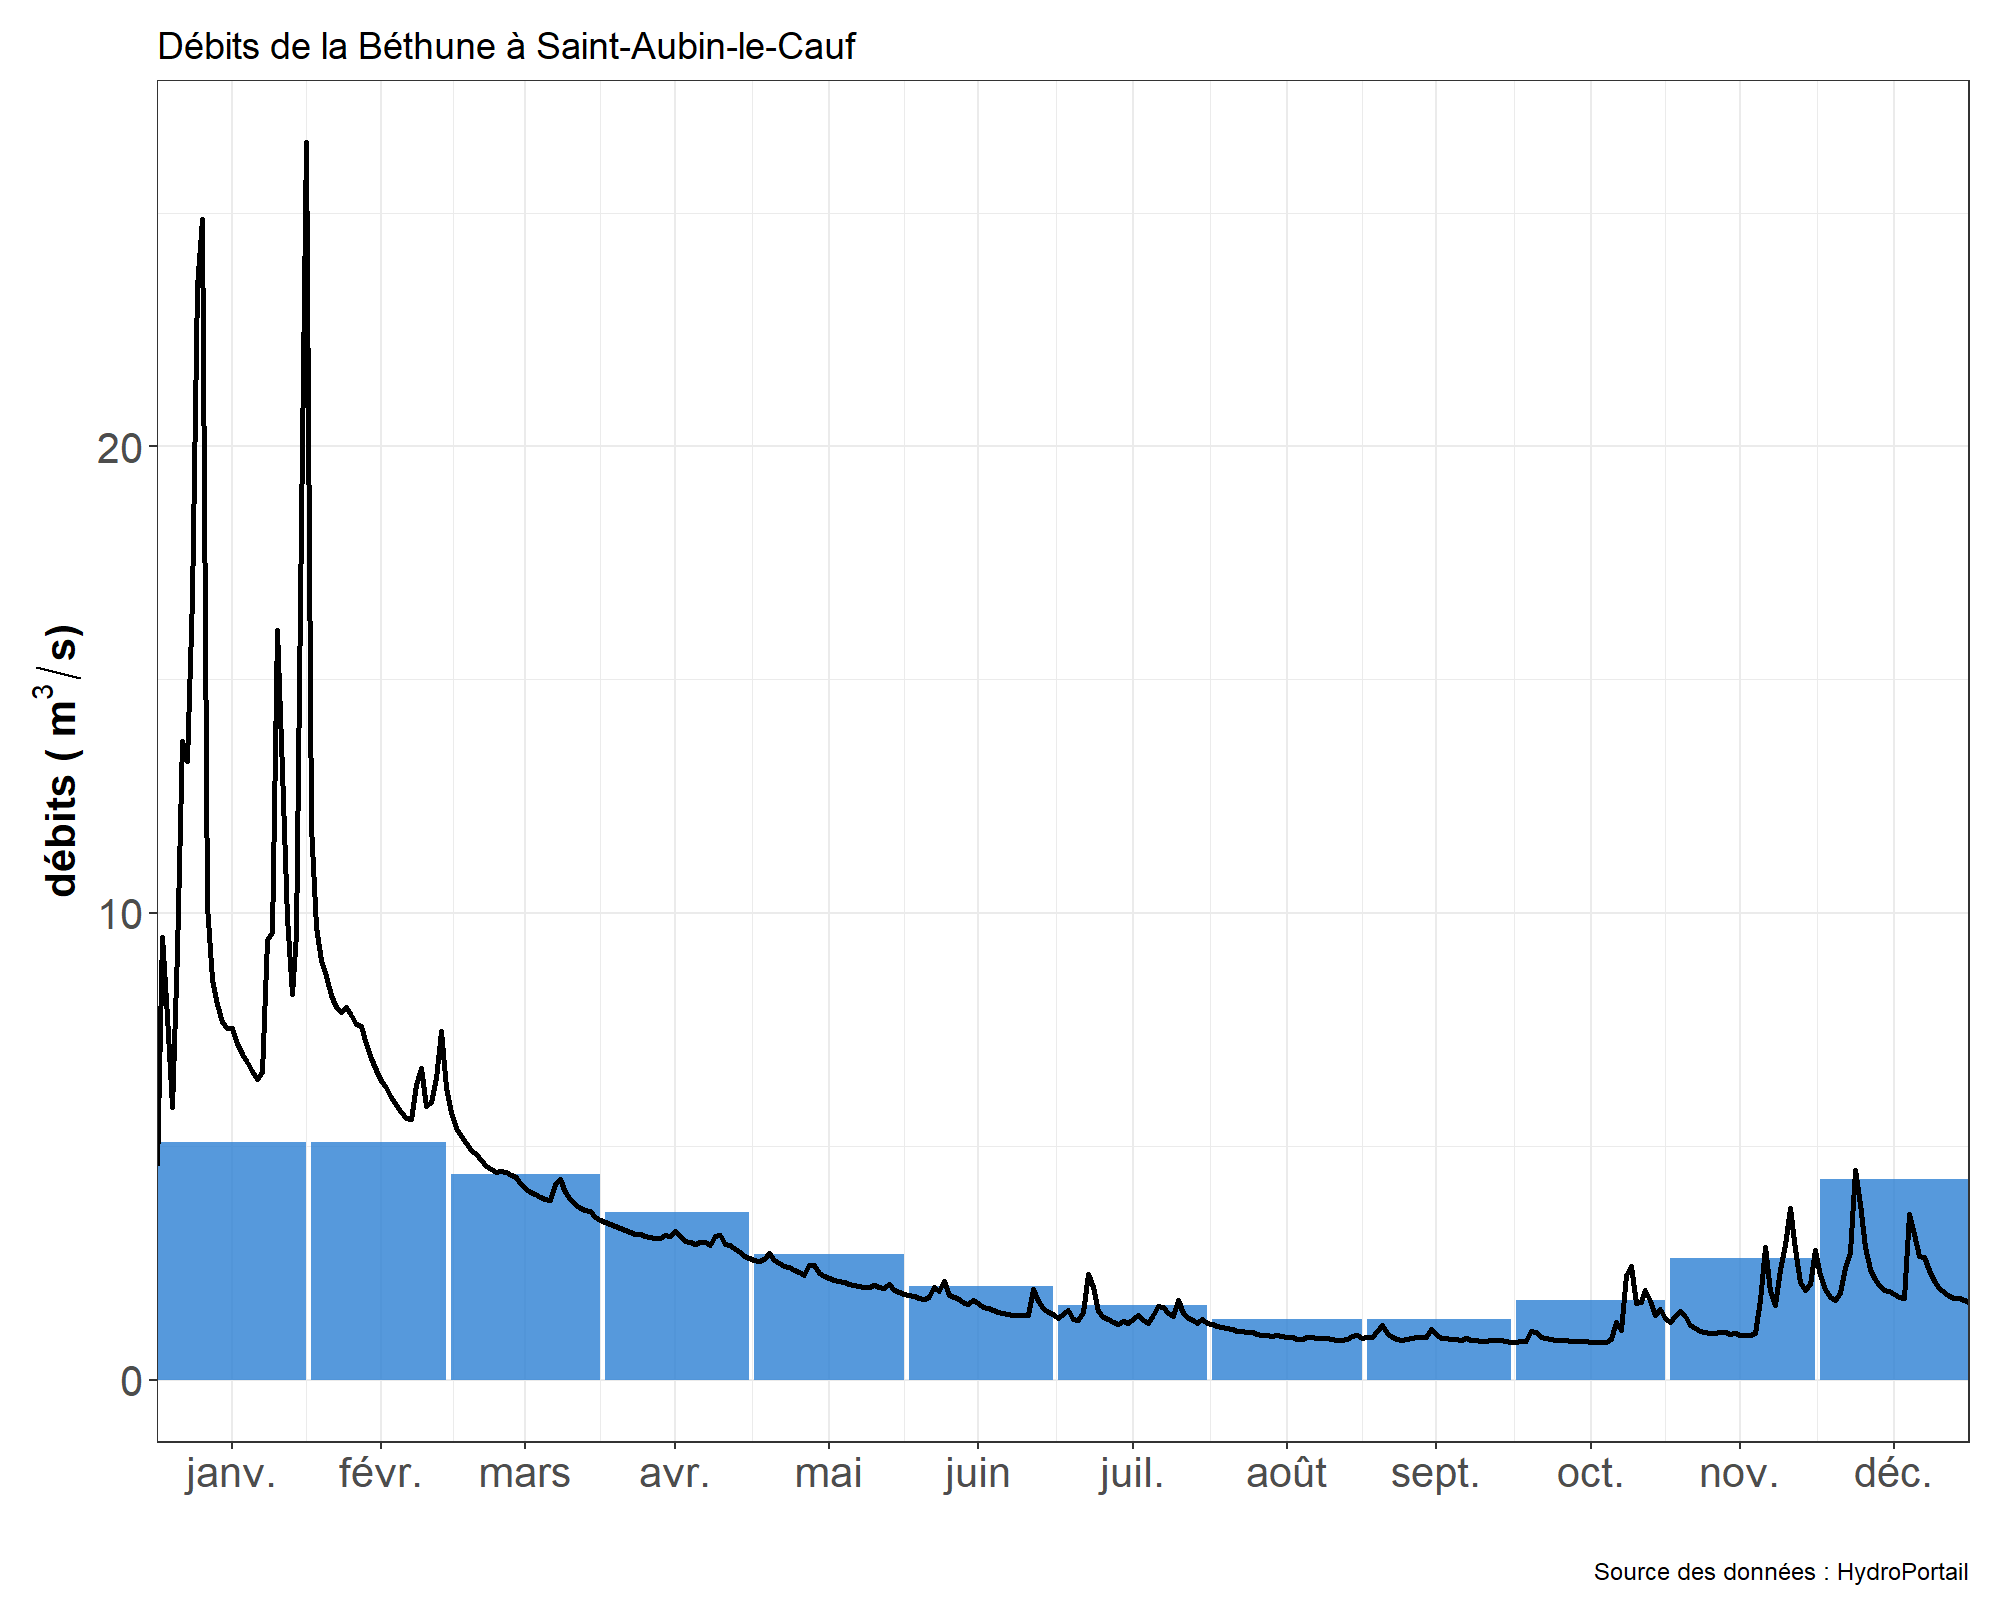
\includegraphics[width=0.8\textwidth]{debit_bethune.png}
\caption{Régime hydrologique de la Seine, de l'Oise et de l'Aisne, le débit moyen mensuel est représenté en bleu, les débits journaliers de l'année sont présentés en noir}
\label{debit_bethune}
\end{figure}
% 
% En tête de bassin, le réseau hydrographique de la Seine traverse quelques massifs cristallins et métamorphiques, notamment dans les Ardennes et le Morvan, avant de s’étendre majoritairement dans la cuvette sédimentaire du bassin parisien. Ce réseau présente les deux extrêmes en matière de densité de cours d'eau, avec des zones fortement densifiées sur les massifs anciens comme dans la Nièvre (58), et des zones crayeuses au drainage peu dense, mais avec un écoulement soutenu et régulier comme en Haute-Normandie.
% 
% La Seine est depuis plusieurs siècles une voie importante de communication et de commerce. Elle présente aujourd'hui 1 427 km de voies navigables, dont 496 km adaptés aux grands gabarits. HAROPA Port est le gestionnaire des ports fluvio-maritimes de la Seine. Il est le premier établissement portuaire de France et le quatrième port nord-européen en tonnage.
% 
% Plus de 18 millions de personnes habitent sur le bassin versant, correspondant à 27 \% de la population nationale, dont 65 \% (11,8 millions) dans la seule région d’Île-de-France. La Seine est considérée comme le fleuve le plus anthropisé de France. Les impacts physico-chimiques (détergents, pesticides...) et morphologiques (artificialisation des berges, chenalisation, édification d'ouvrages...) se ressentent aujourd'hui dans tous les compartiments de l'écosystème, de la source à l'estuaire, jusqu'en baie de Seine.
% 
% \subsection{Situation des poissons grands migrateurs sur la Seine}
% 
% La Seine et ses affluents furent démunis de tous poissons migrateurs, exception faite de l'anguille, pendant plus de 80 ans. Cependant l'application d'un ensemble de mesures de conservation sur les habitats et les espèces, combinée à l'amélioration de la qualité de l'eau via le traitement des effluents ces deux dernières décennies, ont contribué aujourd'hui au retour de presque toutes les espèces migratrices. Les effectifs sont encore modestes par rapport aux populations pristines mais les différents travaux de restauration entrepris ont permis de faire entrer l'hydrosystème de la Seine dans une phase de recolonisation progressive. 
% 
% Les enjeux autour de la conservation des poissons grands migrateurs sont multiples. Ces espèces, de par leur biologie particulière, constituent un patrimoine écologique remarquable. Ces mêmes exigences biologiques et écologiques impliquent une certaine vulnérabilité aux perturbations de l'environnement, à tel point que la majorité des populations sont aujourd'hui menacées.
% 
% C'est par ailleurs logiquement que cette fragilité fait des poissons migrateurs un indicateur pertinent de la qualité des milieux aquatiques qu'ils fréquentent. Leur présence rend compte du bon fonctionnement et du bon état des écosystèmes aquatiques. L'image des migrateurs est d'ailleurs souvent associée à la restauration \og réussie \fg{} des cours d'eau, constituant par conséquent un bon support d'éducation à l'environnement.
% 
% De plus, ces espèces représentent une ressource économique importante pour la pêche professionnelle et/ou amateur. L'Union européenne a montré par exemple que l'exploitation de l'Anguille européenne générait un revenu annuel de l'ordre de 183 millions d'euros.
% 
% Les mesures de conservation et de gestion s'appuient sur la connaissance des populations en place. C'est pourquoi, afin de permettre une recolonisation pérenne des espèces de poissons grands migrateurs dans ce système fluvial, il est indispensable de suivre son évolution. Pour ce faire, il s'agit de s'intéresser aux éléments clés liés aux phases du cycle biologique propres au domaine continental chaque année. Il est donc nécessaire de pouvoir estimer les effectifs migrants en différents points du bassin ; de recenser les frayères actives et d'évaluer le succès reproducteur, comme le fait annuellement la Fédération Départementale des Associations Agréées de Pêche et de Protection des Milieux Aquatiques de l'Eure (FDAAPPMA 27) pour la Lamproie marine sur la Basse-Andelle, l'Eure et l'Epte \citep{sanson_suivi_2009,sanson_suivi_2010,barault_suivi_2013,sanson_suivi_2013}(Figure \ref{photo_lamproies}) et dans l'ensemble d'identifier les zones recolonisées afin de situer les fronts de colonisation sur chacun des axes de migration.
% 
% Les affluents de la Seine estuarienne (la Risle, l'Eure, l'Austreberthe, l'Andelle...) ont notamment un rôle particulier puisque leur proximité immédiate (malgré leur faible linéaire accessible) a permis de maintenir une population de poissons grands migrateurs sur le bassin et ce sont certainement les générations issues de ces populations qui recolonisent le bassin versant.
% 
% \begin{figure}[hptb]
%     \centering
%     \begin{subfigure}[b]{0.45\textwidth}
%         \includegraphics[width=\textwidth]{LPM_tete}
%     \end{subfigure}
%     \begin{subfigure}[b]{0.45\textwidth}
%         \includegraphics[width=\textwidth]{LPM_frayere}
%     \end{subfigure}
%        \caption{A gauche, Lamproie marine à Romilly-sur-Andelle; à droite, Lamproie marine de l'Andelle sur une frayère}
%        \label{photo_lamproies}
% \end{figure}
% 
% \clearpage
% 
% \section{Matériels et Méthodes}
% 
% \subsection{Site de Poses - Amfreville-sous-les-Monts}
% 
% \subsubsection{Barrage}
% 
% Le barrage de Poses représente un point stratégique dans le suivi des effectifs de migration (Figure \ref{reseau_stacomi}). Il s’agit en effet du premier ouvrage sur la Seine, situé à 160 km de la mer, et constituant ainsi le premier point de passage obligatoire pour les migrateurs se dispersant vers l’amont du bassin. La présence d'une station de contrôle des migrations sur cet ouvrage permet aujourd'hui d'identifier et de quantifier les poissons grands migrateurs en montaison chaque année sur l'axe Seine, à l'exception des géniteurs qui trouvent chaque année des zones propices à leur reproduction sur les affluents estuariens cités précédemment.
% 
% Le barrage fut construit en 1885 sur un seuil naturel à des fins de navigation entre les communes de Poses et d'Amfreville-sous-les-Monts (Eure) (Figure \ref{vue_aerienne_poses}). Il fixe la limite de marée dynamique, séparant donc, l'estuaire en aval, de la Seine continentale en amont. Long de 470 mètres, de berge à berge, et présentant une hauteur de chute de 5,4 mètres, l'ensemble de l'ouvrage se décompose en 3 parties : les écluses gérées par Voies Navigables de France (VNF) en rive droite, les vannes sur une distance de 235 mètres, et l'usine hydroélectrique gérée par HYDROWATT en rive gauche.
% 
% \begin{figure}[htpb]
% \centering
% \includegraphics[width=0.8\textwidth]{vue_aerienne_poses}
% \caption{Vue aérienne du barrage et des écluses de Poses - Amfreville-sous-les-Monts}
% \label{vue_aerienne_poses}
% \end{figure}
% 
% \subsubsection{Dispositif de franchissement}
% 
% A la construction de l'usine hydroélectrique en 1991, une passe à poissons a été construite afin de la mettre en conformité vis-à-vis de son installation sur la Seine (Figure \ref{DF_rg_poses}). En effet, au titre de la loi sur l'eau du 16 décembre 1964, tous les ouvrages doivent satisfaire aux exigences de libre circulation piscicole dans les cours d'eau classés, dont la Seine fait partie. Ce classement a été réformé et est aujourd'hui encadré par la Loi sur l'Eau et les Milieux Aquatiques (LEMA).
% 
% La passe est de type passe à bassins à fentes verticales, elle est composée d'un by-pass de dévalaison et de 23 bassins qui s'enchaînent sur une longueur de 86 mètres. En 2013, un dispositif spécifique pour le franchissement des anguilles a été construit (Figure \ref{DF_rg_poses}). Il se découpe en 3 parties :
% 
% - un système aval constitué de 3 rampes de type \og tapis-brosse \fg{} séparées par des bassins de repos ;
% 
% - un canal de liaison d'une longueur de 56 m avec une pente négative (2 \%) ;
% 
% - un dispositif terminal de piégeage.
% 
% \begin{figure}
% \centering
% \includegraphics[width=0.8\textwidth]{DF_rg_poses}
% \caption{Dispositif de franchissement en rive gauche du barrage de Poses - Amfreville-sous-les-Monts. A gauche, passe à bassins à fentes verticales; à droite, rampes de type \og tapis-brosse \fg{}}
% \label{DF_rg_poses}
% \end{figure}
% 
% \begin{figure}
% \centering
% \includegraphics[width=0.8\textwidth]{DF_rd_poses}
% \caption{Dispositif de franchissement en rive droite du barrage de Poses - Amfreville-sous-les-Monts. A gauche, passe à bassins à fentes verticales; à droite, rampes de type \og tapis-brosse \fg{}}
% \label{DF_rd_poses}
% \end{figure}
% 
% En raison de la largeur de la Seine, VNF a construit un deuxième dispositif de franchissement piscicole en rive droite (Figure \ref{DF_rd_poses}) qui vient compléter celui présent au niveau de l'usine hydroélectrique. Cet aménagement est fonctionnel depuis 2017 et se compose d'une passe à poissons et d'une passe à anguilles permettant d'assurer la libre circulation pour l'ensemble des poissons.
% 
% La passe à poissons est également de type passe à bassins à fentes verticales. Elle est constituée de 28 bassins qui s'enchaînent sur une longueur de 60 mètres et une largeur de 28 mètres. La passe à anguilles est constituée en partie aval de deux rampes successives de type \og tapis-brosse \fg{}, séparée par un bassin de repos, amenant à un canal longeant la passe à poissons sur une centaine de mètres et débouchant sur un dispositif de piégeage (Figure \ref{schema_passes}).
% 
% 
% \begin{figure}[hptb]
%     \centering
%     \begin{subfigure}[b]{0.40\textwidth}
%         \includegraphics[width=\textwidth]{schema_passe_rd_poses}
%     \end{subfigure}
%     \begin{subfigure}[b]{0.448\textwidth}
%         \includegraphics[width=\textwidth]{schema_passe_rg_poses}
%     \end{subfigure}
%        \caption{Schémas de la passe à poissons en rive droite (à gauche) et de la passe à poissons en rive gauche (à droite) du barrage de Poses - Amfreville-sous-les-Monts}
%        \label{schema_passes}
% \end{figure}
% 
% \subsection{Site de Pontoise}
% 
% \subsubsection{Barrage}
% 
% L’ouvrage situé sur l’Oise, entre les communes de Pontoise et de Saint-Ouen-l’Aumône, place le dispositif de franchissement et de contrôle à 14 kilomètres de la confluence avec la Seine et à 293 km de la mer. L'obstacle est constitué de deux vannes, avec pour usage principal la navigation, qui génère une hauteur de chute de l’ordre de 1,5 mètre. Propriété de VNF (Voies Navigables de France), son usage a nécessité la construction d’un dispositif de franchissement d’envergure adapté au gabarit de la rivière.
% 
% \subsubsection{Dispositif de franchissement}
% 
% La passe à poissons a été aménagée en rive gauche sur le bras droit de la rivière à l'opposé des écluses de navigation. Composée d’une série de huit bassins à fentes verticales permettant la remontée d’une majorité d’espèces de poissons, une vitre d’observation est en place et a permis l'installation d'un système de vidéocomptage en avril 2023 (Figure \ref{barrage et vc pontoise}). Il permet d'enregistrer les remontées sur cet affluent majeur de la Seine et de statuer, en partie, sur le devenir des individus contrôlés en sortie d’estuaire à Poses-Amfreville-sous-les-Monts.
% 
% \begin{figure}[hptb]
%     \centering
%     \begin{subfigure}[b]{0.4\textwidth}
%         \includegraphics[width=\textwidth]{barrage_pontoise}
%     \end{subfigure}
%     \begin{subfigure}[b]{0.448\textwidth}
%         \includegraphics[width=\textwidth]{chambre_vc_pontoise}
%     \end{subfigure}
%        \caption{Barrage de Pontoise et sa chambre de vidéocomptage}
%        \label{barrage et vc pontoise}
% \end{figure}
% 
% \subsection{Site de Carandeau}
% 
% \subsubsection{Barrage}
% 
% Le barrage de Carandeau est situé sur l'Aisne au niveau de la commune de Choisy-au-Bac dans le département de l’Oise, à seulement 2 km de sa confluence avec l’Oise et à 390 km de la mer. Cet ouvrage a fait l'objet d'une modernisation dans le cadre d'un partenariat signé en 2013 entre Voies navigables de France (VNF) et la société BAMEO, permettant l'automatisation de la gestion du barrage et la restauration de la continuité écologique par l'ajout d'un dispositif de franchissement piscicole (Figure \ref{barrage carandeau}).
% 
% \begin{figure}[htpb]
% \centering
% \includegraphics[width=0.2\textwidth]{carandeau_pap}
% \caption{Dispositif de franchissement en rive droite du barrage de Carandeau}
% \label{barrage carandeau}
% \end{figure}
% 
% \subsubsection{Dispositif de franchissement}
% 
% La passe à poissons est située sur la rive droite et est constituée de 8 bassins successifs à fentes verticales qui se terminent par deux couloirs de comptage. Sa construction a été terminée au cours de l'année 2017 et l'installation du système de comptage a été immédiate. Les obstacles entre la mer et l’aval de l’ouvrage sont tous équipés et théoriquement franchissables. Les informations qu’apporte cette station sont donc très importantes pour évaluer l’efficacité des nouveaux dispositifs à l’aval et pour estimer la recolonisation récente du bassin de l’Aisne par les amphihalins.
% 
% \subsection{Contrôle des migrations}
% 
% Sur le barrage de Poses, les premières années de suivi de la passe à poissons en rive gauche ont été réalisées par le syndicat mixte de la Base de Plein Air et de Loisirs de Léry-Poses. En 2014, à la suite de l’installation de la rampe à anguilles et de son piège, l’association Seine-Normandie Migrateurs a pris en charge son exploitation, puis celle des systèmes de comptage situés en rive droite du barrage lors de leur mise en service en 2018. Depuis 2021, Seinormigr assure également la gestion et le suivi des comptages de la passe à poissons en rive gauche de Poses.
% 
% En 2023, l’association a fait installer un système de comptage sur le barrage de Pontoise, dont elle assure la gestion.
% Le contrôle des migrations au niveau de la passe à poissons de l’ouvrage de Carandeau est, quant à lui, assuré par la Fédération de l’Oise pour la pêche et la protection du milieu aquatique depuis 2018.
% 
% \subsubsection{Dispositif de vidéocomptage}
% 
% Le suivi des migrations piscicoles au niveau des passes à bassins est assuré par un système de vidéocomptage constitué d'une ou deux caméras couplées à un enregistrement informatique à déclenchement automatique (Figure \ref{chambre_vc_poses}). Ce système permet un comptage en continu sans manipulation des poissons, en les faisant passer dans une zone suffisamment visible pour faciliter leur identification et leur dénombrement.
% 
% \begin{figure}[htpb]
% \centering
% \includegraphics[width=\textwidth]{chambre_vc_poses}
% \caption{Chambres de vidéocomptage de la station de contrôle des migrations du barrage de Poses - Amfreville-sous-les-Monts. A gauche, chambre de la rive gauche; à droite, chambre de la rive droite}
% \label{chambre_vc_poses}
% \end{figure}
% 
% Les avantages du comptage numérique sont multiples : absence de manipulation des poissons, possibilité de comptage des espèces difficiles à piéger (comme les aloses), réduction des besoins en personnel par rapport au piégeage, précision élevée pour déterminer les rythmes migratoires et analyser le comportement des différentes espèces.
% 
% Cependant, certaines limites subsistent : impossibilité de comptage en cas de forte turbidité, difficulté de distinguer certaines espèces de petite taille, efficacité variable selon les espèces et sensibilité du système aux objets dérivants (feuilles, herbiers) qui déclenchent des enregistrements parasites.
% 
% Dans les zones où de nombreuses espèces sont présentes une grande partie de l'année, le travail de dépouillement des données vidéo reste relativement lourd et fastidieux.
% 
% \begin{figure}[htpb]
% \centering
% \includegraphics[width=0.8\textwidth]{vc_rd_poses}
% \caption{Schéma du système de vidéocomptage de la station de contrôle des migrations en rive droite du barrage de Poses - Amfreville-sous-les-Monts}
% \label{vc_rd_poses}
% \end{figure}
% 
% \begin{figure}[htpb]
% \centering
% \includegraphics[width=0.8\textwidth]{vc_rg_poses}
% \caption{Schéma du système de vidéocomptage de la station de contrôle des migrations en rive gauche du barrage de Poses - Amfreville-sous-les-Monts}
% \label{vc_rg_poses}
% \end{figure}
% 
% Les dispositifs de vidéocomptage utilisés aux stations de contrôle des migrations de Poses et de Carandeau sont basés sur le système SYSIPAP (CATTOEN, INP-ENSHEEIT) (Figure \ref{vc_rd_poses} et Figure \ref{vc_rg_poses}). Le poisson est amené à s'engager dans un couloir de vision muni de part et d'autre de deux parois vitrées, derrière lesquelles se trouvent en vis-à-vis un rétroéclairage et une caméra filmant ainsi en continu la colonne d'eau où le poisson se présentera.
% 
% La passe à bassins en rive gauche de Poses est munie d'une vitre d'observation tandis que la passe de la rive droite de Poses et celle de Carandeau sont munies d'un double couloir de visualisation permettant de maintenir des vitesses de courant compatibles au franchissement piscicole. Il y a donc deux systèmes de comptage indépendants sur ces sites.
% 
% Lorsqu'un objet transite par un des couloirs de vision, celui-ci est alors détecté par un analyseur d'images qui, selon le seuil de détection qui lui a été imposé, déclenche l'enregistrement, lequel se poursuit tant qu'un objet est toujours visible et/ou détectable. Chaque séquence vidéo est alors stockée dans un serveur de stockage de données informatiques prévu à cet effet.
% 
% Le rôle du système de rétroéclairage disposé derrière la vitre opposée est ainsi d'accentuer le contraste afin de faciliter la détection et la reconnaissance de l'objet. Néanmoins un certain nombre de réglages doivent être appliqués, afin d'étalonner le dispositif en fonction des caractéristiques du site et des espèces de poissons présentes dans le milieu.
% 
% Sur le barrage de Pontoise, le comptage se fait à l'aide du système Ibaï Begi dont le principe de fonctionnement reste identique mais qui permet de fournir des images en haute définition et en couleurs ainsi qu'un système de traitements des vidéos par Intelligence Artificielle. Ce traitement permet de filtrer une partie des séquences générées par des objets dérivants.
% 
% La fiabilité de détection du poisson devant la vitre dépend de divers paramètres de milieu (éclairage, turbidité de l'eau), des espèces de poissons considérées (en fonction de leur taille, de leur couleur, de leur vitesse et de leur profondeur de nage) et de la configuration du site (présence de remous hydrauliques, bullage ou angle mort au niveau de la vitre d'observation). En moyenne, dans de bonnes conditions de visibilité, la fiabilité de détection est excellente (90\% à 100\%) pour les salmonidés, les aloses et les cyprinidés de taille supérieure à 25 cm, bonne (70\% à 90\%) pour les lamproies, barbeaux et cyprinidés de taille comprise entre 10 cm et 25 cm, et moyenne (50\% à 70\%) pour l'anguille et les poissons de taille inférieure à 10 cm \citep{travade_les_1992}.
% 
% Une surveillance régulière est nécessaire pour contrôler les réglages des dispositifs, nettoyer les vitres de visualisation et les zones de passage des poissons.
% 
% \subsubsection{Dépouillement des données de vidéocomptage}
% 
% A la suite de l'enregistrement des séquences vidéo, celles-ci sont visualisées par un opérateur afin d'identifier et de comptabiliser les poissons traversant la passe.
% 
% Les durées de dépouillement sont très variables. En réalité, ces valeurs sont fonctions des conditions de milieu (visibilité, déclenchements parasites par des corps dérivants) et surtout des espèces comptabilisées (facilité de distinction des espèces, vitesse de passage, passages isolés ou en bancs, allers et retours, stabulation devant la vitre, mesure des poissons). A l'expérience des comptages \textit{in situ}, il ressort qu'en moyenne les durées de dépouillement sont de l'ordre de 4 \% à 10 \% du temps réel de surveillance (soit 1 h à 2,5 h par 24 h de suivi) pour les faibles passages (inférieurs à 400 poissons/jour) et de l'ordre de 15 \% à 20 \% du temps réel (soit 3,5 h à 5 h par 24 h de suivi) pour les passages nombreux (3 000 à 5 000 poissons/jour) \citep{travade_les_1992}.
% 
% Tous les poissons franchissant les passes sont identifiés et dénombrés. L’identification est réalisée à l’espèce ou, dans certains cas, à la famille (notamment en présence de passages importants de cyprinidés).
% Les poissons migrateurs sont mesurés sur les stations de Poses et de Pontoise. Un poisson franchissant le couloir de vision en montaison (de l’aval vers l’amont) est noté +1, tandis qu’un individu en dévalaison est noté –1 (par exemple, une anguille argentée dévalante).
% 
% A l'issue du dépouillement, l'ensemble des données est compilé puis importé dans le logiciel \href{http://stacomir.r-forge.r-project.org/}{stacomiR}, qui permet leur traitement et leur analyse. Les données sont consultables via une application \href{https://shiny.seinormigr.fr/Stacomi_App/}{Shiny}.
% 
% \subsubsection{Dispositif de piégeage des anguilles}
% 
% Les systèmes de piégeage sont installés sur la partie amont des dispositifs de franchissement spécifiques aux anguilles. En rive droite, le piège est situé à l’amont du canal à anguilles ; en rive gauche, il se trouve à l’amont du canal de liaison. Ces systèmes sont constitués d'une rampe à \og tapis-brosse \fg{} débouchant sur un vivier (Figure \ref{passe_ang_rd_poses}). L'alimentation de la rampe ainsi que le débit d'attrait sont fournis par une pompe.
% 
% Les dispositifs sont débrayables et mis en service uniquement durant la période de migration des anguilles, c'est-à-dire du mois d'avril jusqu'à l'automne, en fonction des températures de la Seine. Les suivis réalisés sur la passe en rive gauche montrent une reprise de la migration à partir d'une température de 14 $^{\circ}$C \citep{mullet_suivi_2014,lenoir_suivi_2015,flesselle_suivi_2016,sanmartin_suivi_2018}.
% 
% \begin{figure}[htpb]
% \centering
% \includegraphics[width=0.8\textwidth]{passe_ang_rd_poses}
% \caption{Passe piège à anguilles en rive droite du barrage de Poses - Amfreville-sous-les-Monts}
% \label{passe_ang_rd_poses}
% \end{figure}
% 
% \begin{figure}[htpb]
% \centering
% \includegraphics[width=0.8\textwidth]{passe_ang_rg_poses}
% \caption{Passe piège à anguilles en rive gauche du barrage de Poses - Amfreville-sous-les-Monts}
% \label{passe_ang_rg_poses}
% \end{figure}
% 
% \subsubsection{Protocole de suivi}
% 
% Pendant la période de migration, le piège est relevé quotidiennement, hors week-end et jours fériés, sauf en cas de pics migratoires où des relèves supplémentaires peuvent être effectuées. Lors de chaque relève, une biométrie des anguilles est réalisée (Figure \ref{protocole_bio_ang}). Les individus sont préalablement anesthésiés avec une solution d'iso-eugénol avant d'être mesurés (précision 1 mm) et pesés (précision 0,1 g).
% 
% Le protocole de biométrie appliqué varie en fonction de la quantité d'anguilles capturées :
% 
% - Moins de 60 anguilles : biométrie individuelle
% 
% - Entre 60 et quelques milliers d'anguilles : Création de deux lots par tamisage (maille de 6 mm). Pour le lot tamisé, la biométrie est effectuée sur 2 sous-lots de 30 individus et les individus restants sont pesés ensemble. Les individus du refus sont mesurés et pesés individuellement.
% 
% - Plusieurs milliers d'anguilles : Création de 3 lots de 30 individus prélevés aléatoirement, les individus des lots sont biométrés individuellement et le reste des individus est pesé globalement.
% 
% - Pic de migration exceptionnel : Une pesée globale est réalisée et le nombre d'anguilles est estimé en utilisant les données des suivis des jours précédents.
% 
% \begin{figure}[hptb]
%     \centering
%     \begin{subfigure}[b]{0.4\textwidth}
%         \includegraphics[width=\textwidth]{tamis_ang}
%     \end{subfigure}
%     \begin{subfigure}[b]{0.4\textwidth}
%         \includegraphics[width=\textwidth]{biometrie_ang}
%     \end{subfigure}
%        \caption{A gauche, tamisage des anguilles en différents lots de classe de taille; à droite, biométrie des anguilles capturées sur le barrage de Poses - Amfreville-sous-les-Monts}
%        \label{protocole_bio_ang}
% \end{figure}

\clearpage

\section{Suivi des migrations 2025}

\subsection{Anguille européenne (\textit{Anguilla anguilla})}



% Au niveau du barrage de Poses - Amfreville-sous-les-Monts, les anguilles peuvent être contrôlées au niveau des quatre dispositifs de comptage, les deux passes pièges spécifiques à anguille et les deux systèmes de vidéocomptage. Sur les ouvrages de Pontoise et Carandeau, il n'existe pas de rampe spécifique. Les anguilles y sont donc dénombrées uniquement grâce au vidéocomptage.
% 
% Les anguilles empruntant les rampes à brosses sont des jeunes individus (entre 0 et quelques années en eau douce) et en phase de migration active.
% 
% Les individus observés dans les passes à poissons sont soit : 
% 
% – des anguilles jaunes, pouvant être en migration active ou sédentaires (déplacements trophiques, recherche de zones de repos ou d’habitats),
% 
% – des anguilles argentées, qui sont de grands individus en dévalaison effectuant leur migration génésique catadrome.
% Les anguilles jaunes se déplaçant dans les passes à poissons peuvent circuler dans les deux sens (montaison ou dévalaison), ce qui peut conduire certaines années à des sommes de migration négatives (Figure \ref{ANGUILLE}).
% 
% \begin{figure}[htpb]
% \centering
% \includegraphics[width=\textwidth]{ANGUILLE}
% \caption{Anguilles observées au barrage de Poses - Amfreville-sous-les-Monts. A gauche, anguillette capturée dans la passe piège spécifique; au milieu, anguille jaune observée en vidéocomptage; à droite, anguille argentée dévalante observée en vidéocomptage}
% \label{ANGUILLE}
% \end{figure}
% 
% \subsubsection{Anguille en montaison (passe piège) au barrage de Poses}
% 
% En rive droite, les premières arrivées d'anguillettes ont eu lieu le format.Date(min(data_ang_mont_poses_RD_annee$bjo_jour),"%d %B") et les captures se sont terminées le format.Date(max(data_ang_mont_poses_RD_annee$bjo_jour),"%d %B"). Au total, gras(format(round(sum(data_ang_mont_poses_RD_annee$bjo_valeur)),big.mark = " ")) anguilles ont franchi le dispositif de franchissement (Figure \ref{p_ang_mont_poses_RD}).
% 
% En rive gauche, les premières arrivées d'anguillettes ont eu lieu le format.Date(min(data_ang_mont_poses_RG_annee$bjo_jour),"%d %B") et les captures se sont terminées le format.Date(max(data_ang_mont_poses_RG_annee$bjo_jour),"%d %B"). Au total, gras(format(round(sum(data_ang_mont_poses_RG_annee$bjo_valeur)),big.mark = " ")) anguilles ont été comptabilisées sur le dispositif de franchissement (Figure \ref{p_ang_mont_poses_RG}).
% 
% \begin{figure}[htpb]
% \centering
% \includegraphics[width=\textwidth]{p_ang_mont_poses_RD}
% \caption{Rythmes migratoires des anguilles en montaison dénombrées sur la passe piège en rive droite du barrage de Poses - Amfreville-sous-les-Monts}
% \label{p_ang_mont_poses_RD}
% \end{figure}
% 
% \begin{figure}[htpb]
% \centering
% \includegraphics[width=\textwidth]{p_ang_mont_poses_RG}
% \caption{Rythmes migratoires des anguilles en montaison dénombrées sur la passe piège en rive gauche du barrage de Poses - Amfreville-sous-les-Monts}
% \label{p_ang_mont_poses_RG}
% \end{figure}
% 
% Les données historiques montrent des effectifs nettement plus faibles en rive gauche que ceux enregistrés en rive droite, avec une moyenne interannuelle d’environ format(round(mean(subset(data_angmont_histo,station=="Poses rive gauche")$effectif)),big.mark=" ") anguillettes. Une proportion importante de ces individus possède au moins une année de vie continentale (Figure \ref{plot_historique_angmont}). 
% 
% Plusieurs facteurs expliquent les faibles remontées observées en rive gauche :
% 
% – la berge aval de l’ouvrage est constituée de palplanches lisses, ce qui limite la progression des anguilles ;
% 
% – le fort courant généré par les turbines de l’usine hydroélectrique, orienté vers cette berge, rend difficile l’accès aux tapis‑brosses, les anguilles progressant habituellement en utilisant des supports rugueux ;
% 
% – le débit d’attrait de la rampe à anguilles est faible en comparaison de celui induit par le turbinage, rendant la structure difficile à localiser pour les individus.
% 
% Des opérations de capture-marquage-recapture, réalisées depuis 2015, ont permis de confirmer la difficulté pour les anguilles d'accéder à la passe et également de la franchir. En effet, le taux de retour des anguilles marquées et relâchées à 200 mètres en aval de l'ouvrage varie entre 0 \% (en 2018) et 13 \% (en 2015) avec une moyenne de 6,3 \%. Le taux nul observé en 2018 doit être interprété avec prudence, la lecture individuelle des marques devenant particulièrement difficile lorsque les effectifs sont très élevés.
% 
% Le taux de retour des anguilles déposées dans le premier collecteur de la rampe, à la sortie des rampes à brosses, est également faible avec un taux de retour moyen d'environ 45 \%. L'accès et le franchissement de la rampe apparaissent très sélectifs, en particulier pour les jeunes individus disposant de capacités de nage limitées.
% 
% En rive droite, les effectifs observés sont nettement plus importants avec une moyenne interannuelle de format(round(mean(subset(data_angmont_histo,station=="Poses rive droite")$effectif)),big.mark=" ") individus capturés. Cette année encore, les captures confirment la meilleure efficacité de cette rampe, qui fournit des valeurs beaucoup plus représentatives de la situation réelle pour un fleuve du gabarit de la Seine.
% 
% \begin{figure}[htpb]
% \centering
% \includegraphics[width=\textwidth]{plot_historique_angmont}
% \caption{Evolution interannuelle des effectifs des anguilles capturées dans les passes pièges du barrage de Poses - Amfreville-sous-les-Monts}
% \label{plot_historique_angmont}
% \end{figure}
% 
% La phénologie de la migration présente une grande stabilité d’une année à l’autre. Les captures s'intensifient à partir du mois de juin et la majorité des passages se concentrent ensuite en quelques pics intenses corrélés avec des coefficients de marée et qui ont lieu entre mi-juillet et mi-août.
% 
% \begin{figure}[htpb]
% \centering
% \includegraphics[width=0.8\textwidth]{p_seasonal_angmont_poses}
% \caption{Rythmes migratoires des anguilles capturées dans les passes pièges du barrage de Poses - Amfreville-sous-les-Monts.}
% \label{p_seasonal_angmont_poses}
% \end{figure}
% 
% Les tailles des individus capturés s’étendent de min(subset(data_taille_ang_piege, annee == selected_annee)$car_valeur_quantitatif) mm à max(subset(data_taille_ang_piege, annee == selected_annee)$car_valeur_quantitatif) mm, avec une majorité d'anguilles de moins de 100 mm. La taille médiane est de median(subset(data_taille_ang_piege, annee == selected_annee)$car_valeur_quantitatif) mm.
% 
% L'évolution saisonnière des tailles suit le schéma habituel qui voit la taille médiane et l'hétérogénéité des échantillons décroître jusqu'à l'été puis une stabilisation ou une légère hausse de ces variables jusqu'à la fin des suivis (Figure \ref{Taille_ANGMONT}). Celui-ci s'explique par la capture d'individus ayant arrêté leur migration l'année précédente et étant en attente en aval immédiat de l'ouvrage au début de la saison puis l'arrivée progressive des individus de l'année qui vont ensuite faire baisser la taille moyenne de la population piégée.
% 
% \begin{figure}[htpb]
%     \centering
%       \begin{subfigure}[b]{0.48\textwidth}
%           \includegraphics[width=\textwidth]{plot_histo_taille_angmont}
%       \end{subfigure}
%       \begin{subfigure}[b]{0.48\textwidth}
%           \includegraphics[width=\textwidth]{plot_box_violin_plot_angmont}
%       \end{subfigure}
%   \caption{Représentation des tailles des anguilles capturées dans les passes-pièges du barrage de Poses - Amfreville-sous-les-Monts. Les tailles historiques sont présentées en transparence sur les deux graphiques.}
%   \label{Taille_ANGMONT}
% \end{figure}

\clearpage

\subsubsection{Anguille jaune (vidéocomptage)}



% Dans les passes à bassins,les anguilles jaunes observées peuvent être en phase de migration active ou sédentaires, se déplaçant pour rechercher de la nourriture, des habitats ou des zones de repos. Elles peuvent circuler dans les deux sens (montaison et dévalaison). Ainsi, la somme des effectifs comptabilisés peut être négative certaines années. Pour l'année annee, les totaux sont de gras(valeurs_agj_annuelles[1]) à Poses, gras(valeurs_agj_annuelles[2]) Pontoise et gras(valeurs_agj_annuelles[3]) à Carandeau.
% 
% À Pontoise, en raison d'un problème de conception du couloir de vidéocomptage, le comptage des petites espèces, notamment des jeunes anguilles, n'est pas exhaustif. En effet, le radier ne couvre pas l'ensemble du couloir et présente deux voies de passages au niveau des vitres, non couvertes par la caméra, par lesquelles les petits poissons peuvent circuler.
% 
% Il est ainsi fréquent que des anguilles apparaissent directement au milieu du couloir, sans possibilité d'identifier leur sens de migration. Elles sont alors enregistrées dans le logiciel avec un sens \textquote{indéterminé}.
% 
% Les données de cette station ne permettent donc pas de d'estimer un nombre d'anguilles en montaison et doivent donc être considérées à titre informatif. L'espèce est néanmoins bien présente sur cette station, puisque le nombre total d'observations, tous sens de migration confondus (montaison, dévalaison ou indéterminé) atteint format(nrow(subset(bilesp_pontoise,lot_tax_code=="2038" & std_libelle == "Juvénile")),big.mark=" ") individus.
% 
% L'activité est concentrée entre mai et septembre (Figure \ref{plot_annuel_agj}), avec un pic d’intensité au printemps, période correspondant à la hausse saisonnière des températures de l’eau.
% 
% \begin{figure}[htpb]
% \centering
% \includegraphics[width=\textwidth]{plot_annuel_agj}
% \caption{Effectifs journaliers des anguilles jaunes recensés sur les STACOMI du bassin Seine.}
% \label{plot_annuel_agj}
% \end{figure}
% 
% \begin{figure}[htpb]
% \centering
% \includegraphics[width=\textwidth]{plot_historique_agj}
% \caption{Evolution interannuelle des effectifs d'anguille jaune recensés sur les STACOMI du bassin Seine. Les individus dévalants (codés en \textquote{-1}) sont transformés en valeur positive afin de mieux représenter le volume des anguilles ayant transité par les passes à poissons. Les axes des ordonnées n'ont pas la même échelle. Début des comptages : Poses rive gauche en 2008, Poses rive droite et Carandeau en 2018, Pontoise en 2023.}
% \label{plot_historique_agj}
% \end{figure}
% 
% Les données historiques montrent des effectifs variables selon les années, mais globalement compris entre quelques dizaines et quelques centaines d'individus, avec des valeurs logiquement plus importantes à Poses (Figure \ref{plot_historique_agj}).
% 
% Concernant les tailles, les jeunes individus sont majoritaires sur le barrage de Poses. A Pontoise, on observe une proportion importante d'individus < 300 mm, caractéristique des anguilles en phase de migration active.
% 
% L'activité horaire est majoritairement nocturne, conformément au comportement connu de l’espèce (Figure \ref{p_horaires_agj}).
% 
% \begin{figure}[htpb]
% \centering
% \includegraphics[width=\textwidth]{plot_histo_taille_agj}
% \caption{Distribution de tailles des anguilles jaunes mesurées aux stations de Poses et de Pontoise. Les tailles historiques sont présentées en transparence.}
% \label{plot_histo_taille_agj}
% \end{figure}
% 
% \begin{figure}[htpb]
% \centering
% \includegraphics[width=\textwidth,height=0.3\textheight,keepaspectratio]{p_horaires_agj}
% \caption{Horaires de migration des anguilles jaunes en annee}
% \label{p_horaires_agj}
% \end{figure}

\clearpage

\subsubsection{Anguille argentée (vidéocomptage)}



% La production d'anguilles argentées en amont de Poses est estimée, à partir du modèle EDA, à environ 24 000 individus, 5 500 à l'amont de Pontoise et 2 000 à l'amont de Carandeau \citep{briand_eel_2022}. Ces valeurs permettent d’estimer la production générale du bassin, mais le nombre d’individus effectivement contrôlés sur les stations n’est pas représentatif de cette production réelle : seule une fraction des anguilles dévalantes emprunte les passes à poissons. En annee, elles ont été gras(sum(subset(ang_video_agg_annee,station=="Poses")$bjo_valeur)) à être observées à Poses, gras(sum(subset(ang_video_agg_annee,station=="Pontoise")$bjo_valeur)) à Pontoise et gras(sum(subset(ang_video_agg_annee,station=="Carandeau")$bjo_valeur)) à Carandeau.
% 
% Plusieurs voies de franchissement sont en effet disponibles pour les anguilles argentées situées en amont des ouvrages :
% 
% – les passes à poissons,
% 
% – les exutoires de dévalaison,
% 
% – les écluses,
% 
% – les turbines de l’usine hydroélectrique (à Poses),
% 
% – les vannes des barrages.
% 
% Des études menées sur le Gave de Pau \citep{bau_suivi_2012} ont montré que la voie de franchissement utilisée par les anguilles dépend fortement du rapport de débit entre le débit total du cours d'eau et le débit turbiné. Lorsque le débit capté par la turbine dépasse le débit du fleuve, les anguilles franchissent majoritairement l’ouvrage par les turbines. En revanche, lorsque le débit du cours d’eau est au moins 1,5 fois supérieur au débit turbiné, cette voie devient minoritaire.
% 
% Des études menées sur les ouvrages de Seine aval par le bureau d'étude Profish confirment ces conclusions. Les passes à poissons et les écluses n'ont pratiquement pas été utilisées par les anguilles dévalantes marquées et les débits importants semblent favoriser une migration par l'ouvrage plutôt que par les turbines \citep{beguin_suivi_2025}.
% 
% \begin{figure}[htpb]
% \centering
% \includegraphics[width=\textwidth]{plot_annuel_agg}
% \caption{Effectifs journaliers des anguilles argentées recensés sur les STACOMI du bassin Seine.}
% \label{plot_annuel_agg}
% \end{figure}
% 
% \begin{figure}[htpb]
% \centering
% \includegraphics[width=\textwidth]{plot_historique_agg}
% \caption{Evolution interannuelle des effectifs d'anguille argentées recensés sur les STACOMI du bassin Seine. Les axes des ordonnées n'ont pas la même échelle. Début des comptages : Poses rive gauche en 2008, Poses rive droite et Carandeau en 2018, Pontoise en 2023.}
% \label{plot_historique_agg}
% \end{figure}
% 
% \begin{figure}[htpb]
% \centering
% \includegraphics[width=\textwidth,height=0.3\textheight,keepaspectratio]{p_horaires_agg}
% \caption{Horaires de migration des anguilles argentées en annee}
% \label{p_horaires_agg}
% \end{figure}
% 
% La migration de dévalaison est déclenchée par l'augmentation des débits, les passages se concentrent donc durant la période automnale et hivernale (Figure \ref{plot_annuel_agg}).
% 
% Les effectifs dévalants varient selon les années, allant de quelques dizaines à quelques centaines d'individus (Figure \ref{plot_historique_agg}).
% 
% Comme pour les autres stades de l'espèce, la migration de dévalaison se déroule principalement de nuit (Figure \ref{p_horaires_agg}).

\clearpage

\subsection{Lamproie fluviatile (\textit{Lampetra fluviatilis})}



% La lamproie fluviatile est recensée sur le bassin de la Seine (Figure \ref{LPF}), mais cette espèce ne présente pas un comportement de montaison systématique et ses zones de reproduction sont généralement cantonnées sur les parties aval des bassins, en raison notamment de ses capacités de nage et de franchissement limitées. Sa présence n'a donc logiquement jamais été détectée sur les stations de Pontoise et de Carandeau.
% 
% Son dénombrement reste par ailleurs peu significatif sur le barrage de Poses, notamment en rive gauche. En effet, outre la turbidité, le comportement de l'espèce qui effectue des allers-retours devant les vitres entraîne des difficultés de comptage : un individu peut être enregistré en dévalaison sans avoir été détecté lors de sa montaison (passage hors du champ de la caméra ou du côté de la vitre opposée).
% 
% \begin{figure}[htpb]
% \centering
% \includegraphics[width=0.3\textwidth]{LPF_sur_ALA}
% \caption{Lamproie fluviatile, fixée sur une alose, observée en vidéocomptage en rive droite du barrage de Poses - Amfreville-sous-les-Monts.}
% \label{LPF}
% \end{figure}
% 
% phrase_effectif_annuel (Figure \ref{plot_annuel_lpf}). Historiquement à Poses, malgré les difficultés de détection et à titre de comparaison, les données montrent une variabilité assez importante pouvant aller d'une dizaine d'individus jusqu'à plusieurs centaines selon les années (Figure \ref{plot_historique_lpf}). Les faibles observations en rive droite pourraient s'expliquer par les défaillances des organes assurant un débit d'attrait optimal à l'entrée de la passe, problème particulièrement marqué lorsque les débits de la Seine sont élevés.
% 
% \begin{figure}[htpb]
% \centering
% \includegraphics[width=\textwidth]{plot_annuel_lpf}
% \caption{Effectifs journaliers des lamproies fluviatiles recensés sur les STACOMI du bassin Seine.}
% \label{plot_annuel_lpf}
% \end{figure}
% 
% \begin{figure}[htpb]
% \centering
% \includegraphics[width=\textwidth]{plot_historique_lpf}
% \caption{Evolution interannuelle des effectifs de lamproies fluviatiles recensés sur les STACOMI du bassin Seine.}
% \label{plot_historique_lpf}
% \end{figure}
% 
% L'activité migratoire de l'espèce débute tôt dans l'année, les premières montaisons surviennent généralement en janvier, mais il n’est pas rare d’observer des passages encore plus précoces, dès octobre/novembre de l’année précédente (Figure \ref{plot_ridgeline_lpf}). Ces individus précoces sont rattachés à la cohorte de reproduction de l'année suivante. Les individus les plus tardifs peuvent quant à eux franchir l'ouvrage jusqu'au mois d'avril.
% 
% La migration est principalement nocturne, mais des passages en journée sont courants notamment quand la turbidité est importante (Figure \ref{p_horaires_lpf}).
% 
% \begin{figure}[htpb]
% \centering
% \includegraphics[width=0.8\textwidth]{plot_ridgeline_lpf}
% \caption{Rythmes migratoires des lamproies fluviatiles au barrage de Poses - Amfreville-sous-les-Monts.}
% \label{plot_ridgeline_lpf}
% \end{figure}
% 
% \begin{figure}[htpb]
% \centering
% \includegraphics[width=\textwidth,height=0.3\textheight,keepaspectratio]{p_horaires_lpf}
% \caption{Horaires de migration des lamproies fluviatiles en annee}
% \label{p_horaires_lpf}
% \end{figure}

\clearpage

\subsection{Lamproie marine (\textit{Petromyzon marinus})}



% La lamproie marine, autre espèce de la famille des Petromyzontidae, est également recensée sur le bassin de la Seine (Figure \ref{LPM}). Plusieurs sites de reproduction naturelle sont identifiés à ce jour sur des affluents estuariens: l'Eure, l'Andelle et la Risle. Des frayères ont également été observées sur l'Epte, seul affluent de la Seine à l'amont de l'estuaire mais de façon plus ponctuelle.
% 
% \begin{figure}[hptb]
%   \centering
%     \begin{subfigure}[b]{0.3\textwidth}
%         \includegraphics[width=\textwidth]{LPM}
%     \end{subfigure}
%     \begin{subfigure}[b]{0.3\textwidth}
%         \includegraphics[width=\textwidth]{LPM_Pontoise}
%     \end{subfigure}
% \caption{Lamproies marines observées en vidéocomptage à Poses (à gauche) et à Pontoise (à droite).}
% \label{LPM}
% \end{figure}
% 
% La détection de certains individus peut s’avérer difficile, notamment en raison des nombreux allers‑retours effectués devant les caméras, et de conditions de visualisation parfois médiocres en rive gauche (couloir large, bullage important). Malgré cela, l'effectif total de gras(sum(data_lpm_poses_annee$bjo_valeur)) lamproies marines sur l'ensemble du barrage est bien représentatif des effectifs réels ayant réellement franchi l'estuaire (Figure \ref{plot_annuel_lpm}).
% phrase_effectif_pont_carand_lpm
% 
% \begin{figure}[htpb]
% \centering
% \includegraphics[width=\textwidth]{plot_annuel_lpm}
% \caption{Effectifs journaliers des lamproies marines recensés sur les STACOMI du bassin Seine.}
% \label{plot_annuel_lpm}
% \end{figure}
% 
% La lamproie marine était auparavant l'espèce anadrome la plus abondante sur le bassin de la Seine, avec plus d'un millier d'individus franchissant le barrage de Poses jusqu'en 2015 \citep{garot_contromigrations_2015}. Une première chute importante des effectifs est observée à partir de 2016, suivie d’une dégradation encore plus marquée depuis 2023 (Figure \ref{plot_historique_lpm}). Cette tendance est cohérente avec les observations nationales, qui mettent en évidence une baisse généralisée et rapide des populations de lamproie marine \citep{carry_suivi_2017,bgm_site_2019}.
% 
% Les suivis de reproduction réalisés sur les affluents de la Seine aval confirment les données acquises sur les stations de comptage. La situation est aujourd'hui critique pour la survie de l'espèce, tant à l'échelle locale que nationale. Les stations de Carandeau et de Pontoise ayant été mises en service après 2016, leurs observations concernant la lamproie marine demeurent anecdotiques.
% 
% \begin{figure}[htpb]
% \centering
% \includegraphics[width=\textwidth]{plot_historique_lpm}
% \caption{Evolution interannuelle des effectifs des lamproies marines en montaison sur les STACOMI du bassin de la Seine. Les axes des ordonnées n'ont pas la même échelle. Début des comptages : Poses rive gauche en 2008, Poses rive droite et Carandeau en 2018, Pontoise en 2023.}
% \label{plot_historique_lpm}
% \end{figure}
% 
% Au niveau du rythme migratoire, les données historiques montrent des migrations plus tardives que la lamproie fluviatile avec des passages se concentrant entre la fin du mois de mars et juillet avec un pic d'activité ayant lieu entre mai et juin (Figure \ref{plot_seasonal_lpm}).
% 
% La structure de taille des lamproies marines observées en annee est présentée sur la figure \ref{plot_histo_taille_lpm} et comparée à la moyenne
% sur l'ensemble de la série chronologique.
% 
% L'activité horaire est essentiellement nocturne chez cette espèce (Figure \ref{p_horaires_lpm}).
% 
% \begin{figure}[htpb]
% \centering
% \includegraphics[width=\textwidth]{plot_seasonal_lpm}
% \caption{Phénologie de la migration des lamproies marines au barrage de Poses - Amfreville-sous-les-Monts.}
% \label{plot_seasonal_lpm}
% \end{figure}
% 
% \begin{figure}[htpb]
% \centering
% \includegraphics[width=\textwidth,height=0.3\textheight,keepaspectratio]{plot_histo_taille_lpm}
% \caption{Distribution de tailles des lamproies marines mesurées à Poses. Les tailles historiques sont présentées en transparence.}
% \label{plot_histo_taille_lpm}
% \end{figure}
% 
% \begin{figure}[htpb]
% \centering
% \includegraphics[width=\textwidth,height=0.3\textheight,keepaspectratio]{p_horaires_lpm}
% \caption{Horaires de migration des lamproies marines en annee}
% \label{p_horaires_lpm}
% \end{figure}
% 
\clearpage

\subsection{Saumon atlantique (\textit{Salmo salar})}



% Le premier saumon a franchi la passe à poissons le format.Date(min(data_sat_poses_annee$bjo_jour),"%d %B") et le dernier passage a été observé le format.Date(max(data_sat_poses_annee$bjo_jour),"%d %B") (Figure \ref{SAT}). Au total, gras(sum(data_sat_poses_annee$bjo_valeur)) individus ont été recensés en montaison à Poses (Figure \ref{plot_annuel_sat}). phrase_effectif_pont_carand_sat
% 
% \begin{figure}[hptb]
%   \centering
%     \begin{subfigure}[b]{0.3\textwidth}
%         \includegraphics[width=\textwidth]{SAT}
%     \end{subfigure}
%     \begin{subfigure}[b]{0.3\textwidth}
%         \includegraphics[width=\textwidth]{SAT_Pontoise}
%     \end{subfigure}
% \caption{Saumons observés en vidéocomptage à Poses (à gauche) et à Pontoise (à droite).}
% \label{SAT}
% \end{figure}
% 
% 
% \begin{figure}[htpb]
% \centering
% \includegraphics[width=0.8\textwidth]{plot_annuel_sat}
% \caption{Effectifs journaliers des saumons atlantiques observés sur les STACOMI du bassin Seine en annee.}
% \label{plot_annuel_sat}
% \end{figure}
% 
% Lors des premières années de suivi en rive gauche, les effectifs observés avoisinaient en moyenne une soixantaine d’individus, ce qui réduisait fortement la probabilité d’une reproduction significative en amont du bassin.
% La baisse des effectifs enregistrés ces dernières années à la sortie de l’estuaire explique la rareté croissante des observations en amont, tant à Pontoise qu’à Carandeau (Figure \ref{plot_historique_sat}).
% 
% \begin{figure}[htpb]
% \centering
% \includegraphics[width=\textwidth]{plot_historique_sat}
% \caption{Evolution interannuelle des effectifs des saumons atlantiques en montaison sur les STACOMI du bassin de la Seine. Les axes des ordonnées n'ont pas la même échelle. Début des comptages : Poses rive gauche en 2008, Poses rive droite et Carandeau en 2018, Pontoise en 2023.}
% \label{plot_historique_sat}
% \end{figure}
% 
% Au début du suivi sur Poses, les deux vagues présentaient des effectifs équivalents, voire plus importants à l’automne. Ce schéma s’est progressivement inversé, la migration printanière devenant désormais prédominante (Figure \ref{p_seasonal_sat}).
% 
% \begin{figure}[htpb]
% \centering
% \includegraphics[width=0.8\textwidth]{p_seasonal_sat}
% \caption{Rythmes migratoires des saumons atlantiques au barrage de Poses - Amfreville-sous-les-Monts.}
% \label{p_seasonal_sat}
% \end{figure}
% 
% Les tailles mesurées à l'aide du logiciel de dépouillement sont comprises entre round(min(subset(data_taille_sat,annee==selected_annee)$car_valeur_quantitatif)) mm et round(max(subset(data_taille_sat,annee==selected_annee)$car_valeur_quantitatif)) mm, avec une moyenne de round(mean(subset(data_taille_sat,annee==selected_annee)$car_valeur_quantitatif)) mm (Figure \ref{Taille_SAT}).
% 
% Les études scalimétriques ont aidé à démontrer que chez le poisson, hors conditions particulières, la taille d'un individu est corrélée à son âge.
% 
% Ainsi, le saumon peut être classé en trois catégories :
% 
% - les \og castillons \fg{} remontant le fleuve après seulement un hiver en mer dépassent rarement 670 millimètres ;
% 
% - les petits \og saumons de printemps \fg{} séjournent en mer durant deux hivers;
% 
% - les plus vieux individus, dont la taille dépasse 900 mm, qui entreprennent leur migration génésique au terme d'une phase marine d'au moins trois hivers. Ces derniers ne sont pratiquement plus observés sur le bassin.
% 
% \begin{figure}[htpb]
%     \centering
%       \begin{subfigure}[b]{0.48\textwidth}
%           \includegraphics[width=\textwidth]{plot_histo_taille_sat}
%       \end{subfigure}
%       \begin{subfigure}[b]{0.48\textwidth}
%           \includegraphics[width=\textwidth]{plot_age_mer_sat}
%       \end{subfigure}
%   \caption{Représentation des tailles et des âges de mer des saumons atlantiques observés en vidéocomptage au barrage de Poses - Amfreville-sous-les-Monts. Les tailles historiques sont présentées en transparence sur le graphique de gauche.}
%   \label{Taille_SAT}
% \end{figure}
% 
% La migration des saumons est essentiellement diurne (Figure \ref{p_horaires_sat}).
% 
% \begin{figure}[htpb]
% \centering
% \includegraphics[width=\textwidth,height=0.3\textheight,keepaspectratio]{p_horaires_sat}
% \caption{Horaires de migration des saumons atlantiques en annee}
% \label{p_horaires_sat}
% \end{figure}

\clearpage

\subsection{Truite de mer (\textit{Salmo trutta trutta})}



% Le premier individu s'est présenté le format.Date(min(data_trm_poses_annee$bjo_jour),"%d %B") au barrage de Poses, afin d'amorcer la première vague de migration dite \og printanière \fg{} (Figure \ref{TRM}). En effet, au même titre que le saumon, l'activité migratoire de la truite de mer s'articule autour de deux vagues de migration au printemps et à l'automne. Au total, gras(sum(data_trm_poses_annee$bjo_valeur)) individus ont été recensés en montaison à Poses (Figure \ref{plot_annuel_trm}). phrase_effectif_pont_carand_trm
% 
% \begin{figure}[hptb]
%   \centering
%     \begin{subfigure}[b]{0.3\textwidth}
%         \includegraphics[width=\textwidth]{TRM}
%     \end{subfigure}
%     \begin{subfigure}[b]{0.3\textwidth}
%         \includegraphics[width=\textwidth]{TRM_Pontoise}
%     \end{subfigure}
% \caption{Truites de mer observées en vidéocomptage à Poses (à gauche) et à Pontoise (à droite).}
% \label{TRM}
% \end{figure}
% 
% \begin{figure}[htpb]
% \centering
% \includegraphics[width=0.8\textwidth]{plot_annuel_trm}
% \caption{Effectifs journaliers des truites de mer observés sur les STACOMI du bassin Seine en annee.}
% \label{plot_annuel_trm}
% \end{figure}
% 
% La population de truite de mer est historiquement plus abondante que celle du saumon sur le fleuve, ce qui explique des observations plus fréquentes sur les stations en amont, notamment à Carandeau et, plus récemment, à Pontoise (Figure \ref{plot_historique_trm}).
% 
% \begin{figure}[htpb]
% \centering
% \includegraphics[width=\textwidth]{plot_historique_trm}
% \caption{Evolution interannuelle des effectifs des truites de mer en montaison sur les STACOMI du bassin de la Seine. Les axes des ordonnées n'ont pas la même échelle. Début des comptages : Poses rive gauche en 2008, Poses rive droite et Carandeau en 2018, Pontoise en 2023.}
% \label{plot_historique_trm}
% \end{figure}
% 
% Au niveau de la phénologie de la migration et comme chez le saumon, on observe une prédominance croissante de la vague printanière (Figure \ref{p_seasonal_trm}).
% 
% \begin{figure}[htpb]
% \centering
% \includegraphics[width=0.8\textwidth]{p_seasonal_trm}
% \caption{Rythmes migratoires des truites de mer au barrage de Poses - Amfreville-sous-les-Monts.}
% \label{p_seasonal_trm}
% \end{figure}
% 
% Comprise entre round(min(subset(data_taille_trm,annee==selected_annee)$car_valeur_quantitatif)) et round(max(subset(data_taille_sat,annee==selected_annee)$car_valeur_quantitatif)) mm, la taille moyenne de la population atteint round(mean(subset(data_taille_sat,annee==selected_annee)$car_valeur_quantitatif)) mm (Figure \ref{Taille_TRM}).
% 
% Chez la truite de mer, la lecture des écailles (scalimétrie) permet de classer les individus en plusieurs catégories :
% 
% - les finnocks, jeunes individus ayant passé 4 à 6 mois en mer, atteignent rarement 430 mm ;
% 
% - les truites ayant passé un hiver en mer mesurent entre 430 mm et 590 mm ;
% 
% - les individus ayant passé au moins deux hivers en mer peuvent atteindre, voire dépasser, 900 mm. Comme pour le saumon, ces grands individus sont de moins en moins observés sur les stations de comptage.
% 
% \begin{figure}[htpb]
%     \centering
%       \begin{subfigure}[b]{0.48\textwidth}
%           \includegraphics[width=\textwidth]{plot_histo_taille_trm}
%       \end{subfigure}
%       \begin{subfigure}[b]{0.48\textwidth}
%           \includegraphics[width=\textwidth]{plot_age_mer_trm}
%       \end{subfigure}
%   \caption{Représentation des tailles et des âges de mer des truites de mer observées en vidéocomptage au barrage de Poses - Amfreville-sous-les-Monts. Les tailles historiques sont présentées en transparence sur le graphique de gauche.}
%   \label{Taille_TRM}
% \end{figure}
% 
% La migration des truites de mer est majoritairement diurne (Figure \ref{p_horaires_trm}).
% 
% \begin{figure}[htpb]
% \centering
% \includegraphics[width=\textwidth,height=0.3\textheight,keepaspectratio]{p_horaires_trm}
% \caption{Horaires de migration des truites de mer en annee}
% \label{p_horaires_trm}
% \end{figure}


\clearpage

\subsection{Autres espèces}



% Hormis les grands poissons migrateurs, d'autres espèces empruntent les passes à poissons du barrage de Poses, de Pontoise et de Carandeau (Tableau \ref{tab:recap_holobiotique}). L'effectif correspond au nombre de fois où l'espèce a été observée par les caméras, que ce soit en montaison ou en dévalaison. Un effectif égal à zéro indique un poisson observé mais dont le sens de déplacement n’a pas pu être déterminé (apparition ou disparition du poisson au cours de la séquence vidéo).
% 
% \input{table/recap_holobiotique.tex}
% 
% \clearpage

\section{Suivi et fonctionnement technique des dispositifs de contrôle}



% Le fonctionnement des systèmes de franchissement et de comptage dépend de nombreux facteurs, qu’ils soient environnementaux ou matériels, et qui peuvent entraîner des arrêts partiels ou complets des dispositifs. Certains arrêts sont volontaires, notamment pour des opérations de nettoyage des vitres ou de maintenance informatique.
% 
% Les dysfonctionnements les plus courants concernent :
% 
% - les pompes d’alimentation des dispositifs dédiés aux anguilles (alimentation des rampes et débits d’attrait),
% 
% - les problèmes hydrauliques affectant les passes à poissons (ex. : vanne de régulation du débit d’attrait, embâcles),
% 
% - les pannes matérielles ou problèmes logiciels affectant les systèmes de vidéocomptage (onduleur, rétroéclairage).
% 
% Le bilan de l'activité des dispositifs au niveau de la rive gauche de Poses est présenté sur la figure \ref{plot_DC_DF_Poses_RG} et celui de la rive droite est présenté sur la figure \ref{plot_DC_DF_Poses_RD}.
% 
% Comme les années précédentes, le dysfonctionnement majeur sur le barrage de Poses concernait l'attrait de la passe à poissons en rive droite.
% En effet, la vanne de régulation de la sortie hydraulique destinée à maintenir une légère chute ne fonctionnait pas. A cela s'ajoutait un colmatage important de la prise d'eau du canal d'attrait en raison de la panne du dégrilleur, ce qui entraînait une perte de charge dans ce canal et donc une réduction du débit entrant. Des travaux réalisés à partir d'avril ont permis de rétablir la fonctionnalité de la passe à poissons à la fin de l'été. Cette passe a été également été mise en assec au mois de décembre pour effectuer des travaux sur les dispositifs de franchissement et de comptage des anguilles, avec notamment l'installation d'un compteur automatique qui sera opérationnel en 2026.
% 
% \begin{figure}[htpb]
% \centering
% \includegraphics[width=\textwidth,height=0.3\textheight,keepaspectratio]{plot_DC_DF_Poses_RG}
% \caption{Fonctionnement des dispositifs de franchissement et de comptage en rive gauche de Poses.}
% \label{plot_DC_DF_Poses_RG}
% \end{figure}
% 
% \begin{figure}[htpb]
% \centering
% \includegraphics[width=\textwidth,height=0.3\textheight,keepaspectratio]{plot_DC_DF_Poses_RD}
% \caption{Fonctionnement des dispositifs de franchissement et de comptage en rive droite de Poses.}
% \label{plot_DC_DF_Poses_RD}
% \end{figure}
% 
% La fonctionnalité des ouvrages de franchissement et de comptage sur les barrages de Pontoise (Figure \ref{plot_DC_DF_Pontoise}) et de Carandeau (Figure \ref{plot_DC_DF_Carandeau}) a été bonne sur l'ensemble de l'année annee. Le seul arrêt a concerné la fermeture de la passe à poissons de Pontoise pour permettre la réalisation de travaux à l'entrée hydraulique de celle-ci pendant une semaine.
% 
% \begin{figure}[htpb]
% \centering
% \includegraphics[width=0.8\textwidth,height=0.3\textheight,keepaspectratio]{plot_DC_DF_Pontoise}
% \caption{Fonctionnement des dispositifs de franchissement et de comptage à Pontoise.}
% \label{plot_DC_DF_Pontoise}
% \end{figure}
% 
% \begin{figure}[htpb]
% \centering
% \includegraphics[width=0.8\textwidth,height=0.3\textheight,keepaspectratio]{plot_DC_DF_Carandeau}
% \caption{Fonctionnement des dispositifs de franchissement et de comptage à Carandeau.}
% \label{plot_DC_DF_Carandeau}
% \end{figure}

\clearpage

\begin{singlespace}
%\twocolumn
% biblio commune aux différentes années
\bibliographystyle{apalike}
\bibliography{rapport_bethune}
\normalsize
\null
\vfill

Rapport Sweave \LaTeX \\
------------------------\\
packages R : \vspace{1mm}
StacomiR \citep{legrand_stacomir_2019}, hubeau\\
\LaTeX \ :Hmisc, kableExtra, xtable\\
graphiques : ggplot2, patchwork, magick\\
traitements : stringr, lubridate, reshape2, dplyr, plyr, tidyr, questionr, glue\\
------------------------\\
Dernière compilation : le \today \\
 R version 4.6.1 (2026-06-24 ucrt)\\
 plateforme x86-64-w64-mingw32

\clearpage
\end{singlespace}

\end{document}
